\chapter{अनुमापन}\label{ch:g11:titration}

आयरन के एक पूरक का डिब्बा हर गोली में आयरन(II) \omterm{def:g9:ions:ion}{आयनों} के रूप में \qty{80}{mg}
आयरन का वादा करता है। क्या यह सच है? एक रसायनज्ञ गोली को पीसता है,
उसे अम्ल में घोलता है, और एक लंबी अंशांकित नली से पोटैशियम परमैंगनेट का
बैंगनी विलयन बूँद-बूँद करके मिलाता है। हर बूँद तुरंत अपना
रंग खो देती है, क्योंकि परमैंगनेट \omterm{def:g9:ions:ion}{आयन} आयरन(II) \omterm{def:g9:ions:ion}{आयनों} द्वारा खप जाते हैं,
जब तक कि एक बूँद, अंतिम, एक हल्की गुलाबी आभा न छोड़ दे जो फीकी नहीं पड़ती।
उस क्षण तक डाला गया आयतन आयरन की मात्रा बताता है। यह अध्याय
एक अभिक्रिया को एक माप में बदल देता है।

\begin{recall}
\omterm{def:g11:redox:oxidant}{ऑक्सीकारक} \omterm{def:g9:inside-the-atom:nucleus}{इलेक्ट्रॉन} ग्रहण करता है, \omterm{def:g11:redox:oxidant}{अपचायक} उन्हें देता है; परमैंगनेट \omterm{def:g9:ions:ion}{आयन}
आयरन(II) \omterm{def:g9:ions:ion}{आयनों} को इस समीकरण के अनुसार ऑक्सीकृत करता है:
\ce{MnO4^- + 8H+ + 5Fe^{2+} -> Mn^{2+} + 5Fe^{3+} + 4H2O}
(\cref{ch:g11:redox})। \omterm{def:g10:concentration-and-dilution:molar-concentration}{मोलर सांद्रता} और \omterm{def:g10:concentration-and-dilution:dilution}{तनुकरण}
(\cref{ch:g10:concentration-and-dilution}); \omterm{def:g10:reaction-progress-table:extent}{प्रगति सारणी} और
\omterm{def:g10:reaction-progress-table:limiting}{सीमांत अभिकारक} (\cref{ch:g10:reaction-progress-table})।
\end{recall}

\begin{omfigure}
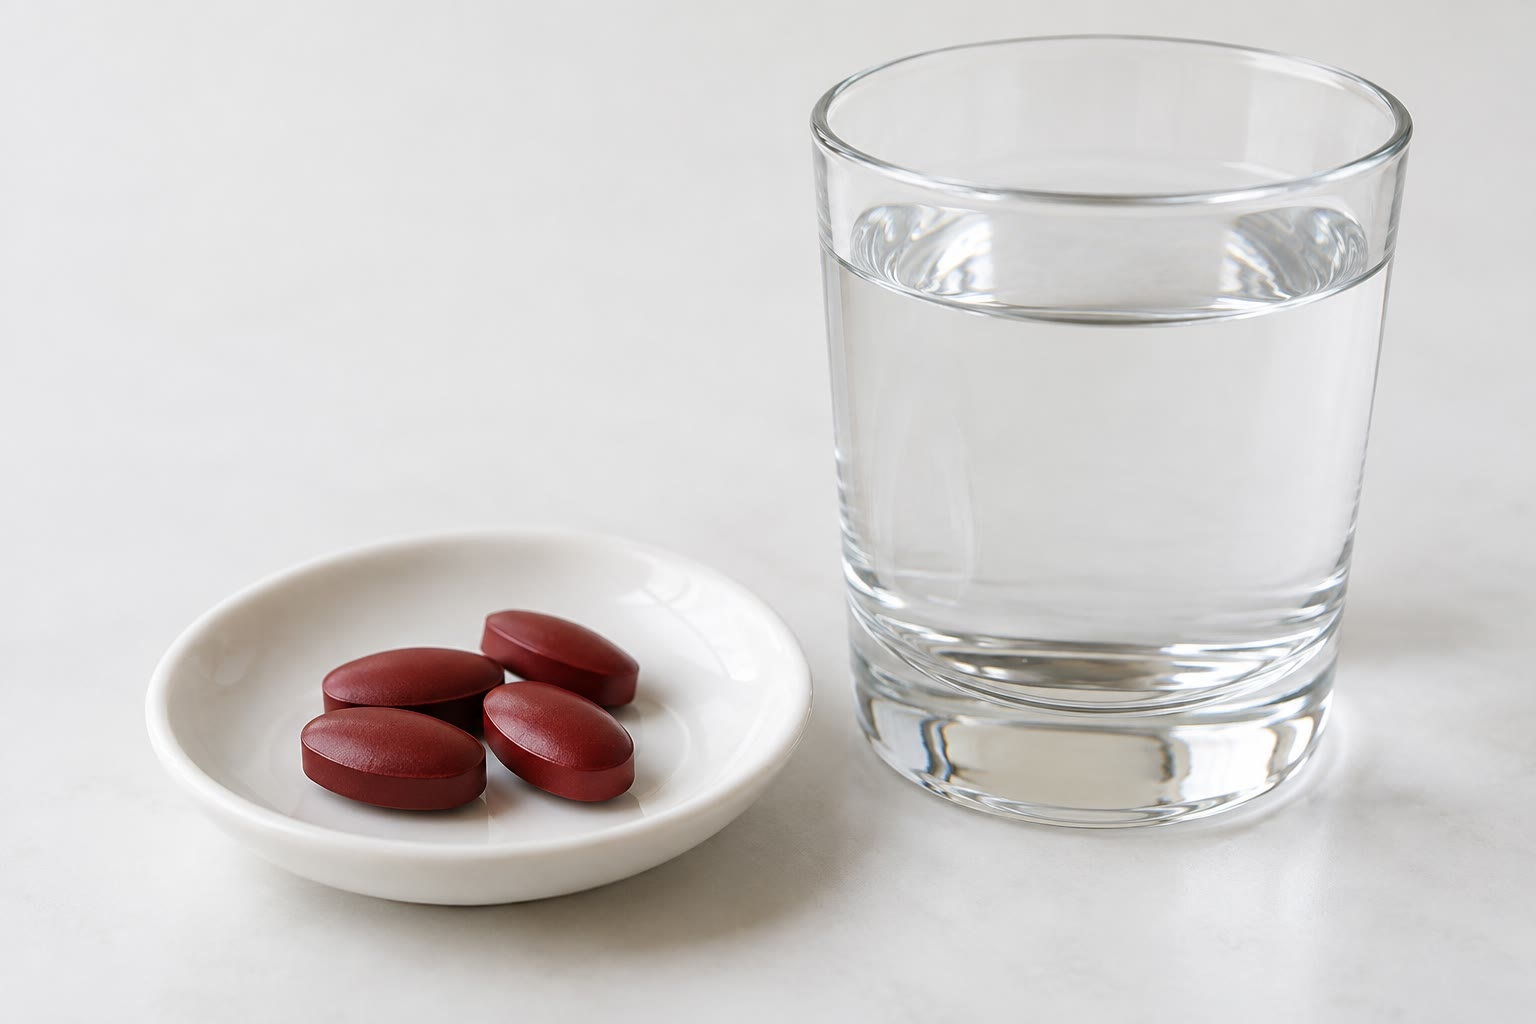
\includegraphics[width=0.45\linewidth]{images/book1/ai/g11-iron-tablets.jpg}

{\small आयरन पूरक की गोलियाँ: हर एक में वास्तव में कितना आयरन है?}
\end{omfigure}

\section{अनुमापन करना}

\begin{definition}[अनुमापन, अनुमापक, अनुमापित विलयन]\label{def:g11:titration:titration}
\emph{अनुमापन}\index{अनुमापन} किसी घुली हुई स्पीशीज़ की मात्रा को
एक ऐसी दूसरी स्पीशीज़ से अभिक्रिया कराकर मापता है जिसकी सांद्रता
सटीक रूप से ज्ञात हो। ब्यूरेट से मिलाया जाने वाला ज्ञात सांद्रता का विलयन
\emph{अनुमापक}\index{अनुमापक} है; फ़्लास्क में रखा, मापी जाने वाली स्पीशीज़
वाला विलयन \emph{अनुमापित
विलयन}\index{अनुमापित विलयन} है।
\end{definition}

\begin{proposition}[अनुमापन अभिक्रिया कैसी होनी चाहिए]\label{prop:g11:titration:conditions}
कोई अभिक्रिया \omterm{def:g11:titration:titration}{अनुमापन} के लिए इस्तेमाल की जा सकती है यदि वह पूर्ण हो (ताकि एक
\omterm{def:g7:chemical-reactions:reactant}{अभिकारक} पूरी तरह खप जाए), तेज़ हो (ताकि हर बूँद तुरंत अभिक्रिया करे),
और एकमात्र हो (\omterm{def:g11:titration:titration}{अनुमापक} फ़्लास्क में किसी और चीज़ से अभिक्रिया न करे)।
\end{proposition}

\begin{proof}
यदि अभिक्रिया पूरी होने से पहले रुक जाती, या बूँदों से पीछे रह जाती,
या \omterm{def:g11:titration:titration}{अनुमापक} को कहीं और खपाती, तो डाला गया आयतन अनुमापित स्पीशीज़ की
मात्रा को अब नहीं मापता।
\end{proof}

\begin{omfigure}
\begin{tikzpicture}[font=\small, scale=0.62]
  \pic[transform shape] at (0,0) {stand={5.8}{1.8}};
  \pic[transform shape] at (1.8,0.68) {stirrer};
  \pic[transform shape] at (1.8,0.68) {erlenmeyer={0.25}{yellow!12}};
  \pic[transform shape] at (1.8,2.98) {burette={0.75}{violet!55}};
  \draw[omProp, thick, <-] (2.15,6.9) -- (4.2,7.4) node[right, text=black,
    align=left] {ब्यूरेट: अनुमापक\\ (पोटैशियम परमैंगनेट)};
  \draw[omProp, thick, <-] (2.55,1.4) -- (4.2,1.9) node[right, text=black,
    align=left] {शंक्वाकार फ़्लास्क: अनुमापित\\ विलयन (आयरन(II), अम्ल)};
  \draw[omProp, thick, <-] (3.0,0.4) -- (4.2,0.3) node[right, text=black]
    {चुंबकीय विलोडक};
\end{tikzpicture}

{\small एक \omterm{def:g11:titration:titration}{अनुमापन} व्यवस्था: स्टैंड पर टिका ब्यूरेट
\omterm{def:g11:titration:titration}{अनुमापक} को \omterm{def:g11:titration:titration}{अनुमापित विलयन} में डालता है, जिसे लगातार हिलाया जाता है।}
\end{omfigure}

\section{तुल्यता}

\begin{definition}[तुल्यता, तुल्यता आयतन]\label{def:g11:titration:equivalence}
\emph{तुल्यता}\index{तुल्यता} \omterm{def:g11:titration:titration}{अनुमापन} का वह क्षण है जब
मिलाया गया \omterm{def:g11:titration:titration}{अनुमापक} और अनुमापित स्पीशीज़ समीकरण के अनुपात में
होते हैं: दोनों खप जाते हैं। उस क्षण तक डाला गया \omterm{def:g11:titration:titration}{अनुमापक} का आयतन
\emph{तुल्यता आयतन}\index{तुल्यता आयतन}, $V_E$, है।
\end{definition}

\begin{proposition}[तुल्यता पर संबंध]\label{prop:g11:titration:relation}
किसी \omterm{def:g11:titration:titration}{अनुमापन} अभिक्रिया $a\,\ce{A} + b\,\ce{B} \longrightarrow$ उत्पाद के लिए, जिसमें A (मात्रा
$n_A$) का \omterm{def:g11:titration:titration}{अनुमापन} सांद्रता $c_B$ वाले \omterm{def:g11:titration:titration}{अनुमापक} B से होता है, \omterm{def:g11:titration:equivalence}{तुल्यता} पर
\[
  \frac{n_A}{a} = \frac{c_B\, V_E}{b} .
\]
\end{proposition}

\begin{proof}
\omterm{def:g11:titration:equivalence}{तुल्यता} पर \omterm{def:g6:pure-substances-and-mixtures:mixture}{मिश्रण} रससमीकरणमितीय होता है
(\cref{ch:g10:reaction-progress-table}): प्रारंभिक मात्राओं $n_A$
और $c_B V_E$ वाले A और B एक साथ समाप्त होते हैं, इसलिए $n_A / a = c_B V_E / b$।
\end{proof}

\begin{omfigure}
\begin{tikzpicture}
\begin{axis}[width=0.72\linewidth, height=5.6cm, xmin=0, xmax=20,
    ymin=0, ymax=16, xlabel={मिलाए गए अनुमापक का आयतन (\si{mL})},
    ylabel={मात्रा ($\num{e-4}$ \si{mol})}, axis lines*=left, ymajorgrids,
    grid style={gray!20}, tick label style={font=\small},
    label style={font=\small}, legend style={font=\small, at={(0.98,0.97)},
    anchor=north east, draw=none}, legend cell align=left]
  \addplot[very thick, orange!70!black, domain=0:14.3] {14.3 - x};
  \addplot[very thick, violet, domain=14.3:20] {0.2*(x - 14.3)};
  \addplot[very thick, violet, domain=0:14.3, forget plot] {0};
  \legend{फ़्लास्क में बचा \ce{Fe^{2+}}, अधिकता में \ce{MnO4^-}}
  \addplot[dashed, black!60] coordinates {(14.3,0) (14.3,7)};
  \node[font=\small, anchor=west] at (axis cs:14.5,6.5) {$V_E = \qty{14.3}{mL}$};
\end{axis}
\end{tikzpicture}

{\small \qty{0.0200}{mol/L} परमैंगनेट द्वारा आयरन(II) का \omterm{def:g11:titration:titration}{अनुमापन}:
आयरन(II) \omterm{def:g9:ions:ion}{आयन} ठीक \omterm{def:g11:titration:equivalence}{तुल्यता आयतन} पर समाप्त होते हैं; उसके बाद
परमैंगनेट \omterm{def:g9:ions:ion}{आयन} अब नहीं खपते और जमा होते जाते हैं।}
\end{omfigure}

\section{रंग-परिवर्तन से तुल्यता का पता लगाना}


\begin{proposition}[तुल्यता देखना]\label{prop:g11:titration:colour}
जब \omterm{def:g11:titration:titration}{अनुमापन} की कोई एक स्पीशीज़ रंगीन होती है, तो \omterm{def:g11:titration:equivalence}{तुल्यता}
फ़्लास्क के रंग-परिवर्तन के रूप में दिखती है: \omterm{def:g11:titration:titration}{अनुमापक} के अधिकता में होते ही उसका रंग प्रकट होकर
बना रहता है, या अनुमापित स्पीशीज़ के समाप्त होने पर उसका रंग
गायब हो जाता है।
\end{proposition}

\begin{proof}
\omterm{def:g11:titration:equivalence}{तुल्यता} से पहले, फ़्लास्क में गिरने वाला \omterm{def:g11:titration:titration}{अनुमापक} का हर \omterm{def:g9:ions:ion}{आयन}
तुरंत खप जाता है; \omterm{def:g11:titration:equivalence}{तुल्यता} के बाद, वह बचा रहता है। इसलिए कोई रंगीन स्पीशीज़
फ़्लास्क में \omterm{def:g11:titration:equivalence}{तुल्यता} के केवल एक ओर ही मौजूद होती है।
\end{proof}

\begin{example}[परमैंगनेट, अपना सूचक स्वयं]\label{ex:g11:titration:permanganate}
परमैंगनेट \omterm{def:g9:ions:ion}{आयन} \ce{MnO4^-} गहरा बैंगनी है, और उससे बनने वाले मैंगनीज़ \omterm{def:g9:ions:ion}{आयन}
\ce{Mn^{2+}} लगभग रंगहीन हैं; आयरन \omterm{def:g9:ions:ion}{आयन} विलयन को केवल
हल्की पीली आभा देते हैं। \omterm{def:g11:titration:equivalence}{तुल्यता} से पहले हर बैंगनी बूँद
गिरते ही रंगहीन हो जाती है; पहली बूँद जो रंगहीन नहीं होती, \omterm{def:g11:titration:equivalence}{तुल्यता}
को चिह्नित करती है: फ़्लास्क हल्का गुलाबी हो जाता है और वैसा ही रहता है।
\end{example}

\begin{omfigure}
\begin{tikzpicture}[font=\small]
  \pic at (0,0) {erlenmeyer={0.3}{yellow!14}};
  \pic at (3.2,0) {erlenmeyer={0.3}{magenta!10}};
  \pic at (6.4,0) {erlenmeyer={0.3}{violet!45}};
  \node[align=center, anchor=north] at (0,-0.15) {तुल्यता से पहले:\\
    हल्का पीला, हर बूँद\\ रंगहीन};
  \node[align=center, anchor=north] at (3.2,-0.15) {तुल्यता पर:\\
    एक हल्की गुलाबी आभा जो\\ बनी रहती है};
  \node[align=center, anchor=north] at (6.4,-0.15) {तुल्यता के बाद:\\
    बैंगनी (परमैंगनेट\\ अधिकता में)};
\end{tikzpicture}

{\small परमैंगनेट द्वारा आयरन(II) के \omterm{def:g11:titration:titration}{अनुमापन} का फ़्लास्क, \omterm{def:g11:titration:equivalence}{तुल्यता} से पहले, उस पर
और उसके बाद। \omterm{def:g11:titration:equivalence}{तुल्यता आयतन} पहली स्थायी गुलाबी आभा पर
पढ़ा जाता है।}
\end{omfigure}

\begin{example}[विटामिन C और आयोडीन]\label{ex:g11:titration:vitamin-c}
% ledger: aw:C, aw:H, aw:O
विटामिन C, ऐस्कॉर्बिक अम्ल \ce{C6H8O6} ($M = \qty{176.0}{g/mol}$), एक
\omterm{def:g11:redox:oxidant}{अपचायक} है; आयोडीन \ce{I2} उसे ऑक्सीकृत करता है:
\[
  \ce{C6H8O6 + I2 -> C6H6O6 + 2H+ + 2I-} .
\]
संतरे के रस के \qty{10.0}{mL} का, थोड़े-से स्टार्च के साथ,
\qty{5.00e-3}{mol/L} के आयोडीन विलयन से \omterm{def:g11:titration:titration}{अनुमापन} किया जाता है। \omterm{def:g11:titration:equivalence}{तुल्यता} से पहले आयोडीन
खप जाता है; अधिकता की पहली बूँद स्टार्च को गहरा नीला कर देती है। यदि
$V_E = \qty{5.70}{mL}$, तो रस में
$n = \num{5.00e-3} \times \num{5.70e-3} = \qty{2.85e-5}{mol}$ विटामिन
C था, अर्थात \qty{10.0}{mL} में \qty{5.0}{mg}: \qty{0.50}{g/L}।
\end{example}

\section{अज्ञात सांद्रता की गणना}

\begin{method}[अनुमापन से सांद्रता की गणना]\label{met:g11:titration:computing}
\begin{enumerate}
  \item \omterm{def:g11:titration:titration}{अनुमापन} अभिक्रिया का \omterm{def:g8:balanced-equations:equation}{संतुलित समीकरण} लिखिए और
        गुणांक $a$ (अनुमापित स्पीशीज़) और $b$ (\omterm{def:g11:titration:titration}{अनुमापक}) पढ़िए।
  \item ब्यूरेट पर $V_E$ पढ़िए, और डाले गए \omterm{def:g11:titration:titration}{अनुमापक} की मात्रा
        $n_B = c_B V_E$ निकालिए।
  \item \omterm{def:g11:titration:equivalence}{तुल्यता} पर, $n_A = \dfrac{a}{b}\, c_B V_E$।
  \item अनुमापित आयतन से भाग दीजिए: $c_A = n_A / V_A$। यदि नमूने का
        \omterm{def:g11:titration:titration}{अनुमापन} से पहले \omterm{def:g10:concentration-and-dilution:dilution}{तनुकरण} किया गया था, तो \omterm{def:g10:concentration-and-dilution:dilution}{तनुकरण गुणांक} से गुणा कीजिए।
\end{enumerate}
\end{method}

\begin{example}[एक आयरन(II) विलयन]\label{ex:g11:titration:iron}
एक अम्लीकृत आयरन(II) विलयन के \qty{20.0}{mL} को \qty{0.0200}{mol/L} के परमैंगनेट के
$V_E = \qty{12.6}{mL}$ की आवश्यकता होती है। यहाँ
$a = 5$ (\ce{Fe^{2+}}) और $b = 1$ (\ce{MnO4^-}):
$n(\ce{MnO4^-}) = 0.0200 \times 0.0126 = \qty{2.52e-4}{mol}$, इसलिए
$n(\ce{Fe^{2+}}) = 5 \times \num{2.52e-4} = \qty{1.26e-3}{mol}$, और
$c(\ce{Fe^{2+}}) = \num{1.26e-3} / 0.0200 = \qty{0.0630}{mol/L}$।
\end{example}

\section{माप के रूप में अनुमापन}

\begin{inthelab}[ब्यूरेट पढ़ना]
ब्यूरेट को \omterm{def:g11:titration:titration}{अनुमापक} से खँगाला जाता है, भरा जाता है, और उसकी नोक को \omterm{def:g4:air-a-mixture-of-gases:air}{हवा} के
बुलबुलों से मुक्त किया जाता है। स्तर को नवचंद्रक के निचले भाग पर पढ़ा जाता है, आँख
उसी ऊँचाई पर रखकर, \omterm{def:g11:titration:titration}{अनुमापन} से पहले और बाद में: डाला गया आयतन
दोनों का अंतर है। अंशांकन हर \qty{0.1}{mL} पर होते हैं, और पाठ्यांक का
\qty{0.05}{mL} तक अनुमान लगाया जा सकता है। \omterm{def:g11:titration:equivalence}{तुल्यता} के निकट \omterm{def:g11:titration:titration}{अनुमापक} बूँद-बूँद
करके मिलाया जाता है, जबकि फ़्लास्क को घुमाया या विलोडित किया जाता है।
\end{inthelab}

\begin{omfigure}
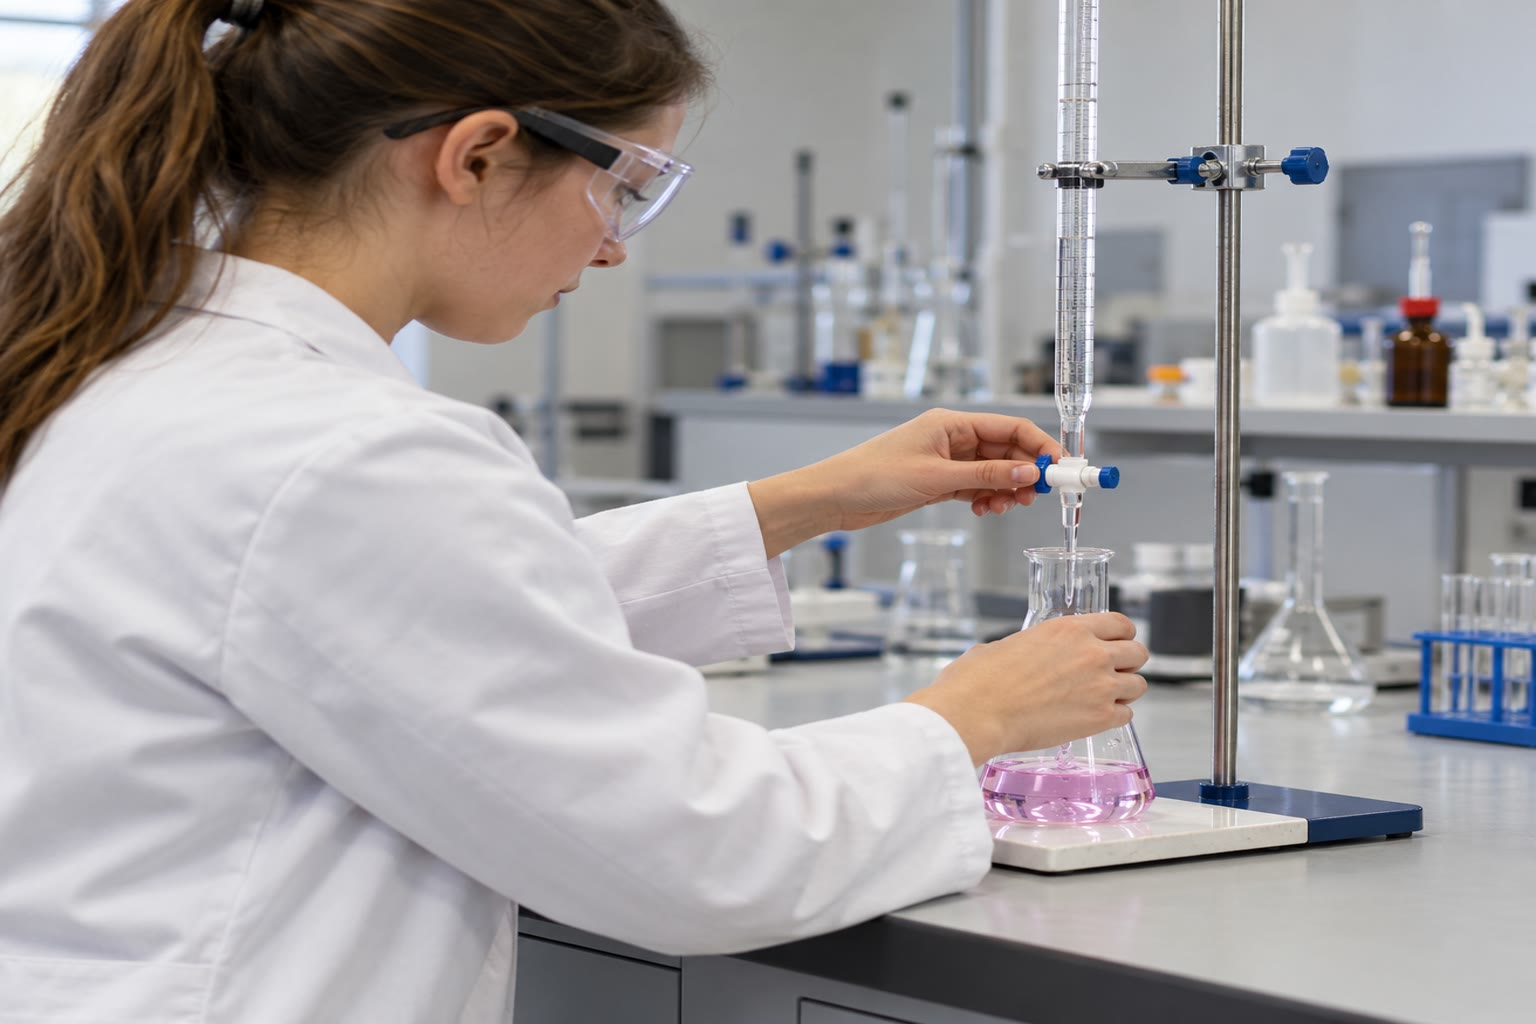
\includegraphics[width=0.48\linewidth]{images/book1/ai/g11-titration-bench.jpg}

{\small चलता हुआ एक \omterm{def:g11:titration:titration}{अनुमापन}: सफ़ेद टाइल पर ब्यूरेट, स्टैंड और शंक्वाकार
फ़्लास्क।}
\end{omfigure}

\begin{remark}[अनुमापन कितना सटीक है?]\label{rem:g11:titration:precision}
ब्यूरेट का हर पाठ्यांक लगभग \qty{0.05}{mL} तक ग़लत हो सकता है, और डाला गया
आयतन दो पाठ्यांकों का अंतर है: \qty{0.1}{mL} तक ग़लत।
$V_E = \qty{14.3}{mL}$ के लिए, यह $0.1 / 14.3 \approx
\qty{0.7}{\percent}$ है। बड़ा $V_E$ इस सापेक्ष त्रुटि को छोटा करता है,
इसीलिए \omterm{def:g11:titration:titration}{अनुमापक} की सांद्रताएँ ऐसी चुनी जाती हैं कि \qty{25}{mL} के ब्यूरेट के साथ
\omterm{def:g11:titration:equivalence}{तुल्यता आयतन} 10 से \qty{20}{mL} के बीच आएँ। \omterm{def:g11:titration:titration}{अनुमापन} तब तक
दोहराया जाता है जब तक दो परिणाम लगभग \qty{0.1}{mL} के भीतर
मेल न खाएँ। किसी माप की अनिश्चितता का अधिक बारीक विवेचन
विश्वविद्यालय के प्रथम वर्ष के खंड में दिया गया है।
\end{remark}

\begin{safety}{\ghs[0.7cm]{GHS03}\ghs[0.7cm]{GHS05}\ghs[0.7cm]{GHS07}\ghs[0.7cm]{GHS08}\ghs[0.7cm]{GHS09}}
% ledger: ghs:KMnO4, ghs:I2
ठोस पोटैशियम परमैंगनेट एक \omterm{def:g11:redox:oxidant}{ऑक्सीकारक} है जो आग को बढ़ा सकता है,
संक्षारक और हानिकारक; उसके तनु विलयन त्वचा और कपड़ों पर भूरे
दाग़ छोड़ते हैं। आयोडीन विलयन हानिकारक हैं। चश्मा और दस्ताने; अपशिष्ट
एकत्र किया जाता है, कभी सिंक में नहीं बहाया जाता।
\end{safety}

\section{अभ्यास}


\begin{exercise}[$\star$]\label{exo:g11:titration:1}
किसी \omterm{def:g11:titration:titration}{अनुमापन} में \omterm{def:g11:titration:titration}{अनुमापक} क्या है? \omterm{def:g11:titration:titration}{अनुमापित विलयन}? \omterm{def:g11:titration:equivalence}{तुल्यता} पर
क्या होता है?
\end{exercise}

\begin{exercise}[$\star$]\label{exo:g11:titration:2}
\qty{0.0200}{mol/L} के विलयन के \qty{12.5}{mL} में परमैंगनेट \omterm{def:g9:ions:ion}{आयनों} की
कितनी मात्रा होती है?
\end{exercise}

\begin{exercise}[$\star$]\label{exo:g11:titration:3}
डाले गए आयतन के विरुद्ध मात्राओं वाले चित्र पर
\omterm{def:g11:titration:equivalence}{तुल्यता आयतन} पढ़िए। शुरुआत में फ़्लास्क में आयरन(II) की कितनी मात्रा
थी?
\end{exercise}

\begin{exercise}[$\star$]\label{exo:g11:titration:4}
परमैंगनेट द्वारा \omterm{def:g11:titration:titration}{अनुमापन} के लिए किसी सूचक की आवश्यकता क्यों नहीं होती?
\end{exercise}

\begin{exercise}[$\star$]\label{exo:g11:titration:5}
परमैंगनेट द्वारा आयरन(II) के \omterm{def:g11:titration:titration}{अनुमापन} की \omterm{def:g11:titration:equivalence}{तुल्यता} पर, आयरन(II) की मात्रा और
डाले गए परमैंगनेट की मात्रा का अनुपात क्या है?
क्यों?
\end{exercise}

\begin{exercise}[$\star\star$]\label{exo:g11:titration:6}
एक अम्लीकृत आयरन(II) विलयन के \qty{10.0}{mL} को \qty{0.0200}{mol/L} के
परमैंगनेट के \qty{8.40}{mL} की आवश्यकता होती है। आयरन(II) की \omterm{def:g10:concentration-and-dilution:molar-concentration}{मोलर सांद्रता}
निकालिए, फिर उसकी \omterm{def:g10:concentration-and-dilution:mass-concentration}{द्रव्यमान सांद्रता}।
\end{exercise}

\begin{exercise}[$\star\star$]\label{exo:g11:titration:7}
विटामिन C की एक गोली को घोलकर \qty{100.0}{mL} विलयन बनाया जाता है।
उसके \qty{10.0}{mL} को, स्टार्च के साथ, \qty{0.0100}{mol/L} के आयोडीन के
\qty{11.4}{mL} की आवश्यकता होती है। गोली में विटामिन C का कितना द्रव्यमान है?
\end{exercise}

\begin{exercise}[$\star\star$]\label{exo:g11:titration:8}
एक अभिक्रिया पूर्ण है पर कई मिनट लेती है। रंग-परिवर्तन वाले \omterm{def:g11:titration:titration}{अनुमापन} के लिए
उसे ज्यों-का-त्यों क्यों इस्तेमाल नहीं किया जा सकता?
\end{exercise}

\begin{exercise}[$\star\star$]\label{exo:g11:titration:9}
तीनों फ़्लास्क देखिए। एक छात्रा तीसरे जितने बैंगनी फ़्लास्क पर रुकती है।
उसका \omterm{def:g11:titration:equivalence}{तुल्यता आयतन} बहुत बड़ा है या बहुत छोटा? \omterm{def:g11:titration:equivalence}{तुल्यता} के निकट
उसे क्या करना चाहिए था?
\end{exercise}

\begin{exercise}[$\star\star$]\label{exo:g11:titration:10}
एक सांद्र आयरन(II) विलयन का पहले दस गुना \omterm{def:g10:concentration-and-dilution:dilution}{तनुकरण} किया जाता है। फिर
तनु विलयन के \qty{10.0}{mL} को \qty{0.0200}{mol/L} के परमैंगनेट के
\qty{13.0}{mL} की आवश्यकता होती है।
सांद्र विलयन की सांद्रता ज्ञात कीजिए।
\end{exercise}

\begin{exercise}[$\star\star$]\label{exo:g11:titration:11}
% ledger: aw:Fe
अध्याय के हल किए गए उदाहरण वाले आयरन(II) विलयन की
$c = \qty{0.0630}{mol/L}$ है। उसके \qty{1.00}{L} में आयरन का कितना द्रव्यमान
होता है?
\end{exercise}

\begin{exercise}[$\star\star\star$]\label{exo:g11:titration:12}
एक \omterm{def:g11:titration:titration}{अनुमापन} $V_E = \qty{7.2}{mL}$ देता है। ब्यूरेट के पाठ्यांकों के कारण सापेक्ष
त्रुटि का अनुमान लगाइए, और $V_E = \qty{14.3}{mL}$ से तुलना कीजिए।
बड़ा \omterm{def:g11:titration:equivalence}{तुल्यता आयतन} पाने के दो तरीके सुझाइए।
\end{exercise}

\begin{exercise}[$\star\star\star$]\label{exo:g11:titration:13}
अम्ल में हाइड्रोजन परॉक्साइड का \omterm{def:g11:titration:titration}{अनुमापन} परमैंगनेट से किया जाता है:
\[
  \ce{2MnO4^- + 5H2O2 + 6H+ -> 2Mn^{2+} + 5O2 + 8H2O} .
\]
एक रोगाणुनाशक का दस गुना \omterm{def:g10:concentration-and-dilution:dilution}{तनुकरण} किया जाता है; तनु विलयन के \qty{10.0}{mL}
को \qty{0.0200}{mol/L} के परमैंगनेट के \qty{17.6}{mL} की आवश्यकता होती है।
रोगाणुनाशक में हाइड्रोजन परॉक्साइड की \omterm{def:g10:concentration-and-dilution:molar-concentration}{मोलर सांद्रता} ज्ञात कीजिए,
फिर उसकी \omterm{def:g10:concentration-and-dilution:mass-concentration}{द्रव्यमान सांद्रता} (\ce{H2O2}: \qty{34.0}{g/mol})।
\end{exercise}

\begin{exercise}[$\star\star\star$]\label{exo:g11:titration:14}
आयरन की एक गोली में लगभग \qty{1.4e-3}{mol} आयरन(II) होना चाहिए।
परमैंगनेट की कौन-सी सांद्रता \qty{25}{mL} के ब्यूरेट के साथ लगभग
\qty{15}{mL} का \omterm{def:g11:titration:equivalence}{तुल्यता आयतन} देती है? दस गुना अधिक सांद्र
विलयन के साथ क्या गड़बड़ होती?
\end{exercise}

\begin{exercise}[$\star\star\star$]\label{exo:g11:titration:15}
\omterm{def:g11:titration:titration}{अनुमापन} के समीकरण में \ce{8H+} आते हैं, प्रत्येक \ce{MnO4^-} के साथ।
\qty{0.0200}{mol/L} पर \qty{14.3}{mL} के \omterm{def:g11:titration:equivalence}{तुल्यता आयतन} के लिए
हाइड्रोजन \omterm{def:g9:ions:ion}{आयनों} की कितनी मात्रा खपती है? क्या
\qty{1.0}{mol/L} हाइड्रोजन \omterm{def:g9:ions:ion}{आयनों} वाले अम्ल के \qty{10}{mL} पर्याप्त हैं? फ़्लास्क को
अम्लीकृत करना क्यों ज़रूरी है?
\end{exercise}

\section{समस्या: क्या आयरन की गोली ईमानदार है?}

\begin{problem}[{सप्ताहांत समस्या --- एक आयरन पूरक प्रति गोली 80 mg
आयरन का दावा करता है: क्या अनुमापन सहमत है?}]
\label{pb:g11:titration:1}
% ledger: aw:Fe, aw:S, aw:O, const:NA
एक आयरन पूरक का डिब्बा प्रति गोली आयरन(II) के रूप में \qty{80}{mg} आयरन का
दावा करता है। एक गोली को पीसकर लगभग \qty{50}{mL}
तनु सल्फ़्यूरिक अम्ल में घोला जाता है, फिर \qty{0.0200}{mol/L} के पोटैशियम परमैंगनेट
से उसका \omterm{def:g11:titration:titration}{अनुमापन} किया जाता है। हल्की गुलाबी आभा $V_E = \qty{14.3}{mL}$ पर बनी रहती है।

\medskip
\noindent\textbf{भाग I --- अभिक्रिया।}
\begin{enumerate}
  \item इसमें शामिल दो \omterm{def:g11:redox:couple}{अपचयोपचय युग्मों} के नाम बताइए। कौन-सी स्पीशीज़
        \omterm{def:g11:redox:oxidant}{ऑक्सीकारक} है, कौन-सी \omterm{def:g11:redox:oxidant}{अपचायक}?
  \item दोनों \omterm{def:g11:redox:couple}{अर्ध-समीकरण} लिखिए।
  \item उन्हें मिलाकर \omterm{def:g11:titration:titration}{अनुमापन} का समीकरण बनाइए, और जाँचिए कि
        वह आवेश में संतुलित है।
  \item गोली को अम्ल में क्यों घोला जाता है?
  \item दिखाइए कि अभिक्रिया \omterm{def:g11:titration:titration}{अनुमापन} की शर्तें पूरी करती है, और
        समझाइए कि \omterm{def:g11:titration:equivalence}{तुल्यता} कैसे दिखती है।
\end{enumerate}

\medskip
\noindent\textbf{भाग II --- \omterm{def:g11:titration:titration}{अनुमापन}।}
\begin{enumerate}[resume]
  \item परमैंगनेट विलयन काँच के किस उपकरण में है? उसका आयतन कैसे
        पढ़ा जाता है?
  \item \omterm{def:g11:titration:equivalence}{तुल्यता} से पहले फ़्लास्क का रंग क्या है, और हर
        बूँद अपना रंग क्यों खो देती है?
  \item \omterm{def:g11:titration:equivalence}{तुल्यता} पर डाले गए परमैंगनेट की मात्रा निकालिए।
\end{enumerate}

\medskip
\noindent\textbf{भाग III --- आयरन।}
\begin{enumerate}[resume]
  \item गोली में आयरन(II) की मात्रा निकालिए।
  \item उसका द्रव्यमान मिलीग्राम में निकालिए।
  \item लेबल से तुलना कीजिए: सापेक्ष अंतर?
  \item डाला गया आयतन \qty{0.1}{mL} तक ग़लत हो सकता है। आयरन का द्रव्यमान कितने
        मिलीग्राम तक ग़लत हो सकता है? क्या लेबल की पुष्टि होती है?
\end{enumerate}

\medskip
\noindent\textbf{भाग IV --- कई गोलियाँ।}
\begin{enumerate}[resume]
  \item दो और गोलियाँ $V_E = \qty{14.1}{mL}$ और
        \qty{14.4}{mL} देती हैं। उनके आयरन के द्रव्यमान निकालिए।
  \item तीनों गोलियों का माध्य निकालिए।
  \item तीनों परिणाम ब्यूरेट की त्रुटि से अधिक भिन्न हैं। इससे
        गोलियों के बारे में क्या पता चलता है?
  \item क्या \qty{0.100}{mol/L} का परमैंगनेट बेहतर
        विकल्प होता? समझाइए।
  \item कई पूरकों में विटामिन C भी होता है, जो एक \omterm{def:g11:redox:oxidant}{अपचायक} है। वह \omterm{def:g11:titration:titration}{अनुमापन} पर
        और ज्ञात किए गए आयरन के द्रव्यमान पर क्या प्रभाव डालेगा?
  \item आयरन, आयरन(II) सल्फ़ेट, \ce{FeSO4}, के रूप में मौजूद है। एक गोली में उसका
        कितना द्रव्यमान है?
  \item यह कितने आयरन(II) \omterm{def:g9:ions:ion}{आयन} हैं?
  \item अंतिम उत्तर बताइए: एक गोली में आयरन का कितना द्रव्यमान
        है?
\end{enumerate}
\end{problem}
